%%%%%%%%%%%%%%%%%%%%%%%%
%%%%% EXPERIMENTS %%%%%%
%%%%%%%%%%%%%%%%%%%%%%%%
\section{Experiments}
\label{sec:experiments}
Herein, we evaluate the performance of the proposed method (referred to as \texttt{DenseReg}) on various face-related tasks. 
%The experiments are performed on challenging publicly available benchmarks and we report substantial improvements over the current state-of-the-art. 
In the following sections, we first describe the training setup (Sec.~\ref{sec:training_setup}) and then present extensive quantitative results on \emph{(i)}~semantic segmentation (Sec.~\ref{sec:exp_semantic_segmentation}), \emph{(ii)}~landmark localization on static images (Sec.~\ref{sec:exp_landmark_localization}), \emph{(iii)}~deformable tracking (Sec.~\ref{sec:exp_deformable_tracking}), \emph{(iv)}~ dense correspondence on human bodies (Sec.~\ref{sec:exp_human}), and \emph{(v)}~human ear landmark localization (Sec.~\ref{sec:exp_ear}).
%Finally, we report qualitative results on \emph{(v)}~depth estimation (Sec.~\ref{sec:exp_depth}) and \emph{(vi)}~3D shape estimation (Sec.~\ref{sec:exp_mm}), for which it is not possible to provide quantitative evaluation due to lack of established benchmarking. 
%We note that DenseReg is not trained or fine-tuned specifically for each one of those tasks. Its predictions are  used out-of-the-box the different task-specific evaluations. 
Due to space constraints, we refer to the supplementary material for additional qualitative results, experiments on monocular depth estimation and further analysis of experimental results.


%%%%%%%%%%%%%%%%%%%%%%%%%%%%%%%
%%%%%%% TRAINING SETUP %%%%%%%%
%%%%%%%%%%%%%%%%%%%%%%%%%%%%%%%
\subsection{Training Setup}
\label{sec:training_setup}

\textbf{Training Databases for Faces.} We train our system using the 3DDFA data of \citep{zhu2016face}. The 3DDFA data provides projection and 3DMM model parameters for the Basel \citep{paysan20093d} + FaceWarehouse \citep{cao2014facewarehouse} model for each image of the 300W database. We use the topology defined by this model to define our UV space and rasterize the images to obtain per-pixel ground truth UV coordinates.  Our training set consists of the LFPW trainset, Helen trainset and AFW, thus 3148 images
that are captured under completely unconstrained conditions
and exhibit large variations in pose, expression, illumination,
age, etc.
 Many of these images contain multiple faces, some of which are not annotated. We deal with this issue by employing the out-of-the-box DPM face detector of Mathias et al.~\citep{mathias2014face} to obtain the regions that contain a face for all of the images. The detected regions that do not overlap with the ground truth landmarks do not contribute to the loss. For training and testing, we have rescaled the images such that their largest side is 800 pixels.
 
 \textbf{Training Databases for Bodies}
 
 In order to create the supervisor UV signals for the body we made use of the recently proposed \textit{Unite the People} (UP)~\citep{lassner2017unite} dataset. The data is formed by automatically fitting the SMPL 3D model~\citep{loper2015smpl} (which has components that describe both the shape and the articulation of the human body in dense 3D). 
 %
 For our experiments on human pose estimation with the cascaded architecture, in order to have a dense supervisory signal for all of the MPII and LSP images, we used the code provided by \citep{lassner2017unite}, to fit the SMPL model by minimizing the energy function proposed in ~\citep{bogo2016keep}. Even though some fits are erroneous, which are filtered in the UP dataset, the incorporation of dense correspondences yield improved pose estimation results. We used the estimated 3D shape and camera parameters to render a pixel-vertex correspondence map, where each image pixel is labeled with the corresponding vertex index and compute the corresponding UV maps. 
 
 The pose estimation experiments were performed on two well known body pose databases: MPII Human Pose \citep{andriluka20142d} and Leeds Sport Poses (LSP) + extended training set \citep{Johnson10}. There are around 18k training images and 7k testing images involved in MPII. We split training set randomly to make a 3k size validation set while the rest are used for training. Results on LSP are reported by fine tuning the same model with the 11k extended LSP training set.

\textbf{CNN Training for DenseReg} 

We have used two different network architectures for our experiments. In particular, in order to be directly comparable to the DeepLab-v2 network in semantic segmentation experiments we first used a ResNet101~\citep{He2015} architecture with dilated convolutions ( atrous )~\citep{CP2015Semantic,mallat1999wavelet}, such that the stride of the CNN is $8$ and (b) an Hourglass-type network \cite{newell2016stacked}. We use bilinear interpolation to upscale both the $\hat{q}$ and $\hat{r}$ branches before the losses. The losses are applied at the input image scale and back-propagated through interpolation. We apply a weight to the smooth $L1$ loss layers to balance their contribution. In our experiments, we have used a weight of $40$ for quantized~($d=0.1$) and a weight of $70$ for non-quantized regression, which are determined by a coarse cross validation. 

For the ResNet based network, we use an initialization with a network pre-trained for the MS COCO segmentation task~\citep{lin2014microsoft}. The new layers are initialized with random weights drawn from Gaussian distributions. Large weights of the regression losses can be problematic at initialization even with moderate learning rates. To cope with this, we use initial training with a lower learning rate for a \textit{warm start} for a few iterations. We then use a base learning rate of $0.001$ with a polynomial decay policy for $20k$ iterations with a batch size of $10$ images.

For the hourglass architecture, we adopt \cite{newell2016stacked} with inception-v2 module (a Figure describing the network can be found in the Appendix). Each deconvolution layer involved is using a dilated convolution following by a $3\times 3$ convolution layer with stride 1 and same output channels as input channels. 


\textbf{CNN Training for DenseReg Cascade} 

For the DenseReg cascade architecture (i.e., end-to-end trainable dense shape regression and articulated pose estimation by means of landmark localisation) we used a stack of two hourglasses. The first hourglass network is the one described above. The second hourglass network is regressing to a  heatmap representation of facial landmarks/body joints (68-channel heatmap for the landmark localisation experiments and 16-channel heatmap of the body pose estimation experiments). We apply $L2$ loss to the heatmap regression. Weights are applied to balance losses of both first and second hourglasses to have equal contribution. During training, we are randomly scaling with ratio between 0.75 and 1.25, randomly rotating with angle -30 to 30 degree, and randomly cropping images of size $321\times321$ to $256\times256$.

%%%%%%%%%%%%%%%%%%%%%%%%%%%%%%%%%%
%%%%% SEMANTIC SEGMENTATION %%%%%%
%%%%%%%%%%%%%%%%%%%%%%%%%%%%%%%%%%
\subsection{Semantic Segmentation}
\label{sec:exp_semantic_segmentation}
% \vspace{-0.35cm}

As discussed in Sec.~\ref{sec:SDMs}, any labelling function defined on the template shape can be transferred to the image domain using the regressed coordinates. One application that can be naturally represented on the template shape is semantic segmentation of facial parts. 
To this end, we manually defined a segmentation mask of $8$ classes  (right/left eye, right/left eyebrow, upper/lower lip, nose, other) on the template shape, as shown in Fig.~\ref{fig:Semantic}. 
%%%%%%%%%%%%%%%%%%%%%%%%%%%%%%%%%%%%%%%%
\begin{figure}[h]
\vspace{-0.25cm}
\centering
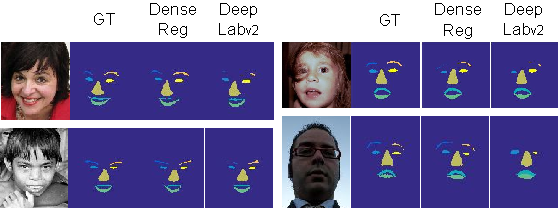
\includegraphics[width=\linewidth ]{Figures/segs-3}
\caption{Exemplar semantic segmentation results.}
\label{fig:Semantic}
\vspace{-0.25cm}

\end{figure}
%%%%%%%%%%%%%%%%%%%%%%%%%%%%%%%%%%%%%%%%

We compare against a state-of-the-art semantic part segmentation system (DeepLab-v2)~\citep{CP2016Deeplab} which is based on the same ResNet-101 architecture as our proposed DenseReg. We train DeepLab-v2 on the same training images (i.e. LFPW trainset, Helen trainset and AFW).  We generate the ground-truth segmentation labels for both training and testing images by transferring the segmentation mask using the ground-truth deformation-free coordinates explained in Sec.~\ref{sec:SDMs}. We employ the Helen testset~\citep{le2012interactive} for the evaluation.

Table~\ref{tab:Semantic} reports evaluation results using the intersection-over-union (IoU) ratio. Additionally, Fig.~\ref{fig:Semantic} shows some qualitative results for both methods, along with the ground-truth segmentation labels. The results indicate that the DenseReg outperforms DeepLab-v2. The reported improvement is substantial for several parts, such as eyebrows and lips. We believe that this result is significant given that DenseReg is not optimized for the specific task-at-hand, as opposed to DeepLab-v2 which was trained for semantic segmentation. This performance difference can be justified by the fact that DenseReg was exposed to a  richer label structure during training, which reflects the underlying variability and structure of the problem. 

%%%%%%%%%%%%%%%%%%%%%%%%%%%%%%%%%%%%%%%%

\begin{table}[h]
\centering
\begin{tabular}{|l|cc|}
\hline
\emph{Class} & \emph{Methods}& \\
\cline{2-3}
 & \textbf{DenseReg}  & Deeplab-v2 \\
\hline\hline
Left Eyebrow     & 48.35 & 40.57\\
Right Eyebrow    & 46.89 & 41.85\\
Left Eye         & 75.06 & 73.65\\
Right Eye        & 73.53 & 73.67\\
Upper Lip        & 69.52 & 62.04\\
Lower Lip        & 75.18 & 70.71\\
Nose             & 87.71 & 86.76\\
Other            & 99.44 & 99.37\\
\hline\hline
Average          & \textbf{71.96} & 68.58\\
\hline
\end{tabular}
\caption{Semantic segmentation accuracy on Helen testset measured using intersection-over-union (IoU) ratio.}
\vspace{-0.05cm}
\label{tab:Semantic}
\end{table}
%%%%%%%%%%%%%%%%%%%%%%%%%%%%%%%%%%%%%%%%

% We create a segmentation testing dataset by transferring the segmentation mask visualized in Fig.1 using the ground-truth deformation-free coordinates to the images.

% A standard way to approach this problem, given a dataset of segmented face parts, would be to use a fully convolutional neural network trained to classify each pixel. The alternative we propose is to transfer the labels to the image domain using the regressed coordinates. Using the segmentation ground-truth labels obtained, we train a state of the art semantic segmentation network based on ResNet-101\citep{Newdeeplab} architecture. Results from all three methods are visualized in Fig.~\ref{fig:Semantic} and the intersection-over-union measure for each class for both approaches are presented in Tab.\ref{tab:Semantic}. The results indicate that the dense regression framework does better on this task compared to the segmentation network. Even though our network was not optimized specifically for this task, it was exposed to a much richer label structure which explains the better performance.



%%%%%%%%%%%%%%%%%%%%%%%%%%%%%%%%%%
%%%%% LANDMARK LOCALIZATION %%%%%%
%%%%%%%%%%%%%%%%%%%%%%%%%%%%%%%%%%
\captionsetup[subfigure]{labelformat=empty}


\begin{figure*}[h]
\centering

\subfloat{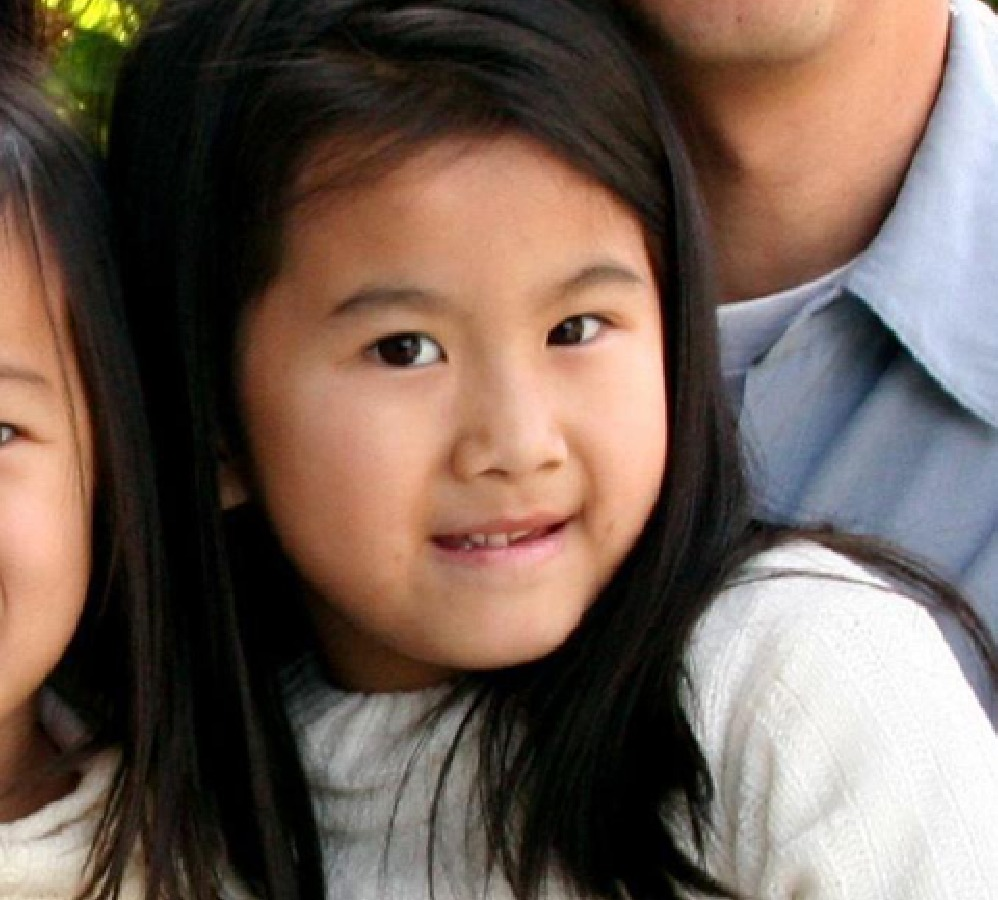
\includegraphics[width=0.13775\textwidth]{Figures/Results/1/I}}\hspace{0.0005cm}
\subfloat{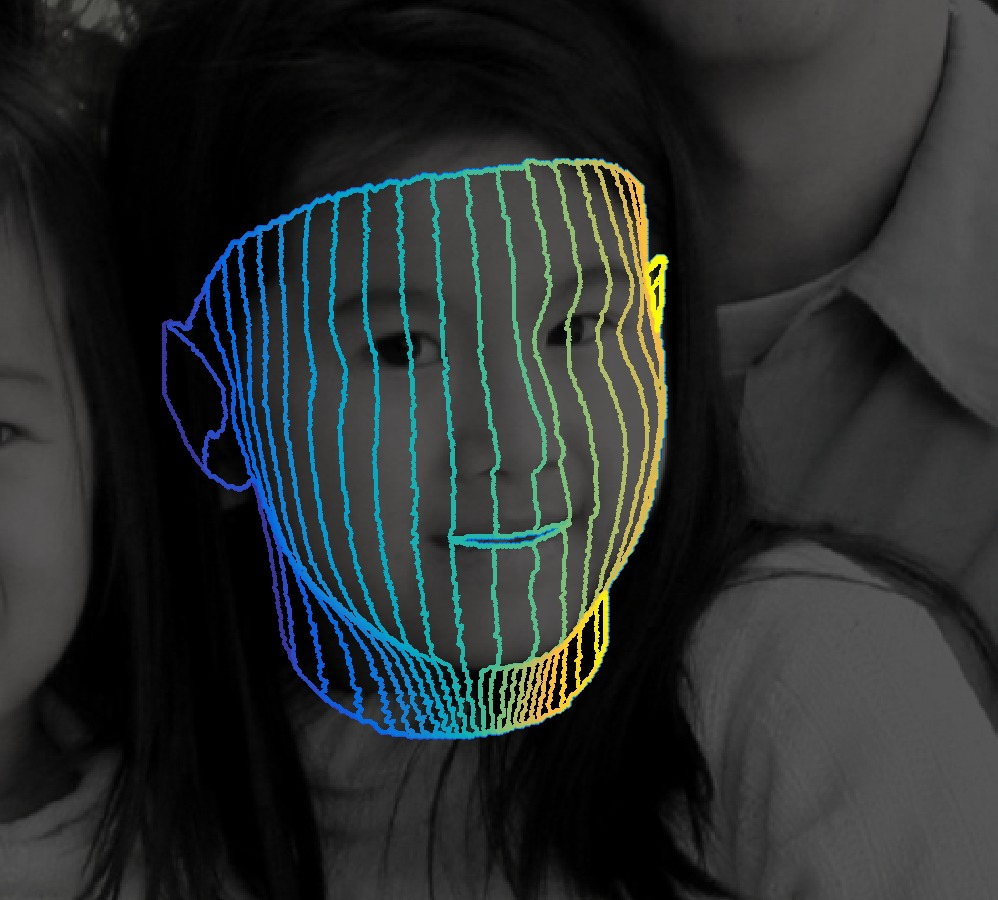
\includegraphics[width=0.13775\textwidth]{Figures/Results/1/HGT}}\hspace{0.0005cm}
\subfloat{\includegraphics[width=0.13775\textwidth]{Figures/Results/1/Hreg}}\hspace{0.0005cm}
\subfloat{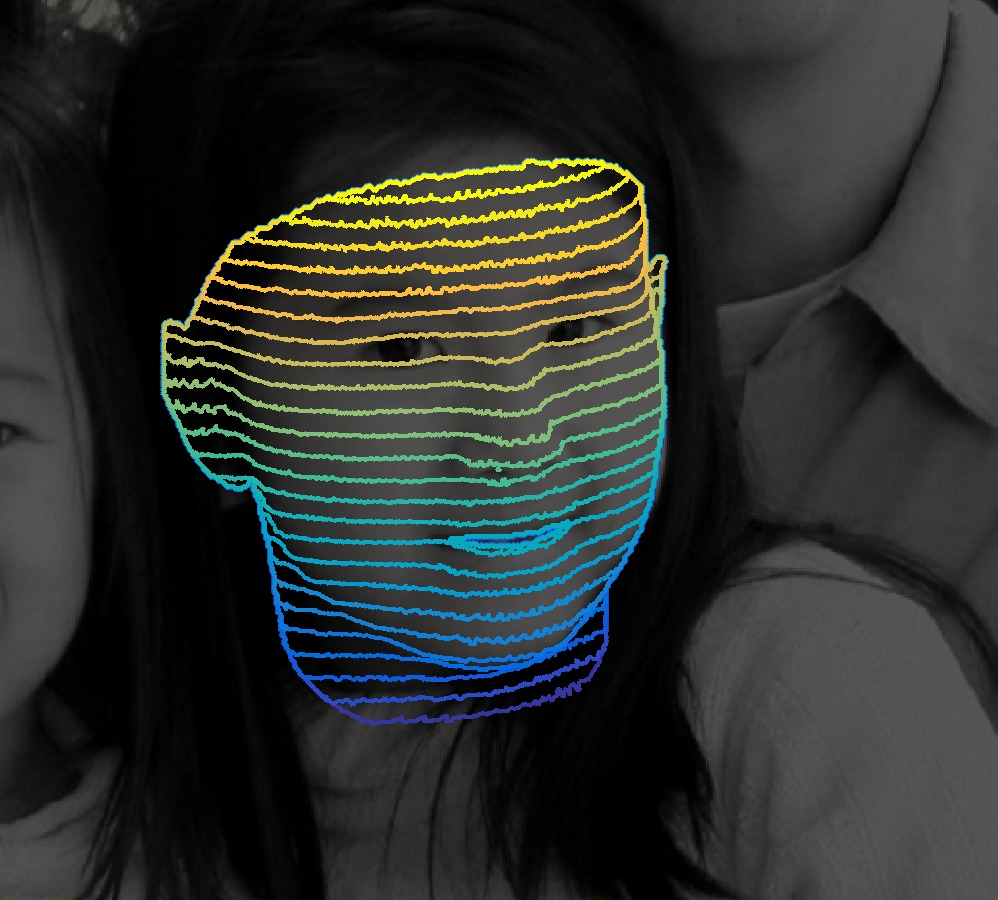
\includegraphics[width=0.13775\textwidth]{Figures/Results/1/VGT}}\hspace{0.0005cm}
\subfloat{\includegraphics[width=0.13775\textwidth]{Figures/Results/1/Vreg}}\hspace{0.0005cm}
\subfloat{\includegraphics[width=0.13775\textwidth]{Figures/Results/1/Landmarks_alp}}\hspace{0.0005cm}
\subfloat{\includegraphics[width=0.13775\textwidth]{Figures/Results/1/Landmarks_MDM}}\\
\vspace{-0.3cm}
% \vspace{-0.3cm}
\subfloat{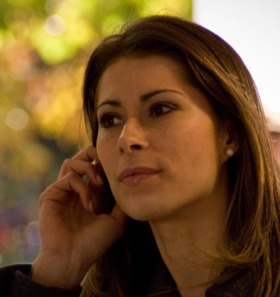
\includegraphics[width=0.13775\textwidth]{Figures/Results/3/I}}\hspace{0.0005cm}
\subfloat{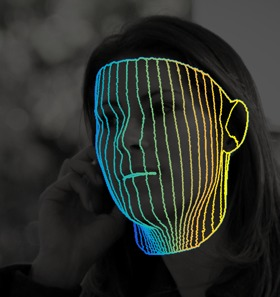
\includegraphics[width=0.13775\textwidth]{Figures/Results/3/HGT}}\hspace{0.0005cm}
\subfloat{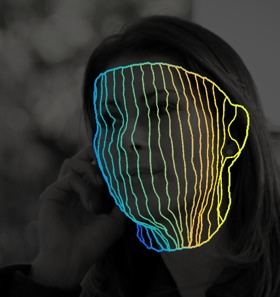
\includegraphics[width=0.13775\textwidth]{Figures/Results/3/Hreg}}\hspace{0.0005cm}
\subfloat{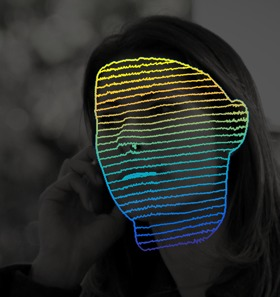
\includegraphics[width=0.13775\textwidth]{Figures/Results/3/VGT}}\hspace{0.0005cm}
\subfloat{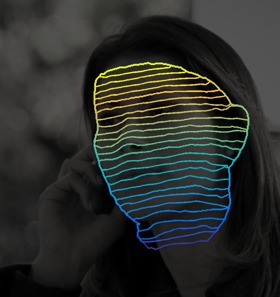
\includegraphics[width=0.13775\textwidth]{Figures/Results/3/Vreg}}\hspace{0.0005cm}
\subfloat{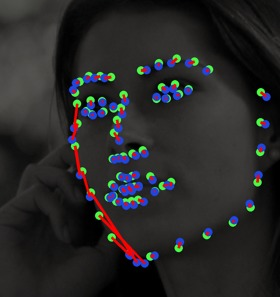
\includegraphics[width=0.13775\textwidth]{Figures/Results/3/Landmarks_alp}}\hspace{0.0005cm}
\subfloat{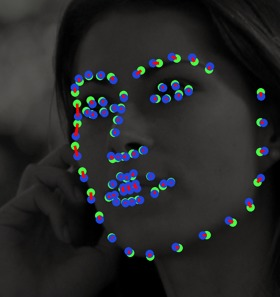
\includegraphics[width=0.13775\textwidth]{Figures/Results/3/Landmarks_MDM}}\\
%
\vspace{-0.3cm}
\subfloat[Input Image]{\includegraphics[width=0.13775\textwidth]{Figures/Results/7/I}}\hspace{0.0005cm}
\subfloat[Groundtruth~$U$~$u^h$ ]{\includegraphics[width=0.13775\textwidth]{Figures/Results/7/HGT}}\hspace{0.0005cm}
\subfloat[Estimated~$U$~$\hat{u}^h$ ]{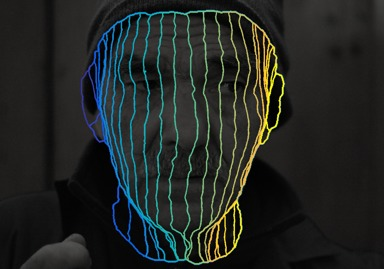
\includegraphics[width=0.13775\textwidth]{Figures/Results/7/Hreg}}\hspace{0.0005cm}
\subfloat[Groundtruth~$V$~$u^v$]{\includegraphics[width=0.13775\textwidth]{Figures/Results/7/VGT}}\hspace{0.0005cm}
\subfloat[Estimated~$V$~$\hat{u}^v$]{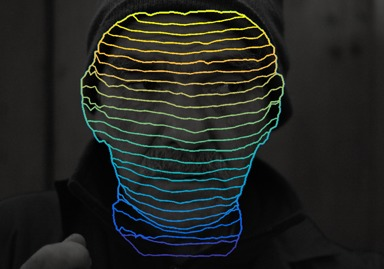
\includegraphics[width=0.13775\textwidth]{Figures/Results/7/Vreg}}\hspace{0.0005cm}
\subfloat[DenseReg]{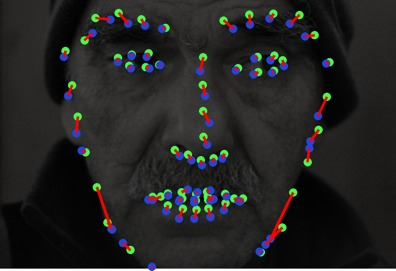
\includegraphics[width=0.13775\textwidth]{Figures/Results/7/Landmarks_alp}}\hspace{0.0005cm}
\subfloat[DenseReg+MDM]{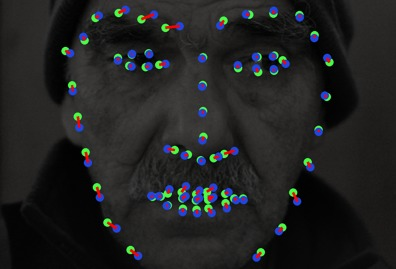
\includegraphics[width=0.13775\textwidth]{Figures/Results/7/Landmarks_MDM}}\\
\vspace{-0.13cm}

% \subfloat{\includegraphics[width=0.13775\textwidth]{Figures/Results/8/I}}\hspace{0.0005cm}
% \subfloat{\includegraphics[width=0.13775\textwidth]{Figures/Results/8/HGT}}\hspace{0.0005cm}
% \subfloat{\includegraphics[width=0.13775\textwidth]{Figures/Results/8/Hreg}}\hspace{0.0005cm}
% \subfloat{\includegraphics[width=0.13775\textwidth]{Figures/Results/8/VGT}}\hspace{0.0005cm}
% \subfloat{\includegraphics[width=0.13775\textwidth]{Figures/Results/8/Vreg}}\hspace{0.0005cm}
% \subfloat{\includegraphics[width=0.13775\textwidth]{Figures/Results/8/Landmarks_alp}}\hspace{0.0005cm}
% \subfloat{\includegraphics[width=0.13775\textwidth]{Figures/Results/8/Landmarks_MDM}}\\

\caption{Qualitative Results. Ground-truth and estimated deformation-free coordinates and  landmarks obtained from DenseReg and DenseReg+MDM are presented. Estimated landmarks(blue), ground-truth(green), lines between estimated and ground-truth landmarks(red).}
\label{fig:qualitative}
\vspace{-0.3cm}

\end{figure*}

\subsection{Landmark Localization on Static Images}
\label{sec:exp_landmark_localization}

%%%%%%%%%%%%%%%%%%%%%%%%%%%%%%%%%%%%%%%%
\begin{figure}[!b]
\vspace{-0.25cm}
\centering
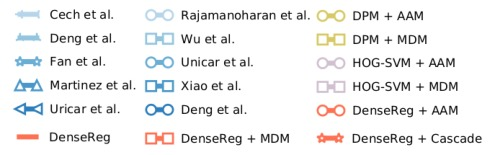
\includegraphics[width=0.9\linewidth]{Figures/legend_all}
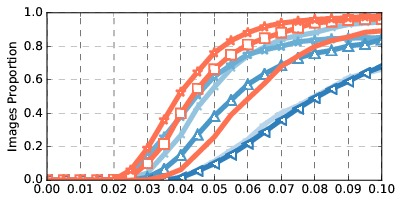
\includegraphics[width=0.9\linewidth]{Figures/300w_68}
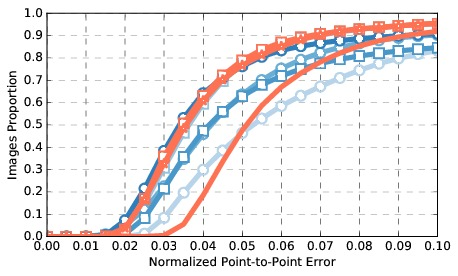
\includegraphics[width=0.9\linewidth]{Figures/300vw_all}
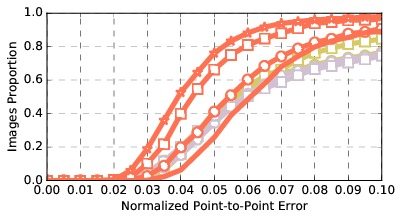
\includegraphics[width=0.9\linewidth]{Figures/300w_selfevaluation}
\caption{Landmark localization results using 68 points. Accuracy is reported as Cumulative Error Distribution of RMS point-to-point error normalized with interocular distance. \emph{Top:} Comparison with state-of-the-art on the 300W testing dataset. \emph{Middle:} Comparison with state-of-the-art on the 300WV tracking dataset.\emph{Bottom:} Self-evaluation results on the 300W testing dataset.}
\vspace{-0.15cm}
\label{fig:300w}
\end{figure}
%%%%%%%%%%%%%%%%%%%%%%%%%%%%%%%%%%%%%%%%

DenseReg can be readily used for the task of facial landmark localization on static images. Given the landmarks' locations on the template shape, it is straightforward to estimate the closest points in the deformation-free coordinates on the images. The local minima of the Euclidean distance between the estimated coordinates and the landmark coordinates are considered as detected landmarks. In order to find the local minima, we simply analyze the connected components separately. Even though more sophisticated methods for covering ``touching shapes'' can be used, we found that this simplistic approach is sufficient for the task. 

Note that the closest deformation-free coordinates among all \emph{visible} pixels to a landmark point is not necessarily the correct corresponding landmark. This phenomenon is called ``landmark marching''~\citep{zhu2015high} and mostly affects the jaw landmarks which are dependent on changes in head pose. It should be noted that we do not use any explicit supervision for landmark detection nor focus on ad-hoc methods to cope with this issue. Errors on jaw landmarks due to invisible coordinates and improvements thanks to deformable models can be observed in Fig.~\ref{fig:qualitative}.

Herein, we evaluate the landmark localization performance of DenseReg as well as the performance obtained by employing DenseReg as an initialization for deformable models~\citep{papandreou2008adaptive,tzimiropoulos2014gauss,antonakos2015feature,trigeorgis2016mnemonic} trained for the specific task. In the second scenario, we provide a slightly improved initialization with very small computational cost by reconstructing the detected landmarks with a PCA shape model that is constructed from ground-truth annotations. 


We present experimental results using the very challenging 300W benchmark. This is the testing database that was used in the 300W competition~\citep{sagonas_iccv_300w_2013,sagonas2016300} - the most important facial landmark localization challenge. The error is measured using the point-to-point RMS error normalized with the interocular distance and reported in the form of Cumulative Error Distribution (CED). Figure~\ref{fig:300w} (bottom) presents some self-evaluations in which we compare the quality of initialization for deformable modelling between DenseReg \footnote{We have tested both the ResNet and the hourglass-based architecture and the provided the same results, hence we will not present them separately.} and two other standard face detection techniques (HOG-SVM~\citep{king2015max}, DPM~\citep{mathias2014face}). The employed deformable models are the popular generative approach of patch-based Active Appearance Models (AAM)~\citep{papandreou2008adaptive,tzimiropoulos2014gauss,antonakos2015feature}, as well as the current state-of-the-art approach of Mnemonic Descent Method (MDM)~\citep{trigeorgis2016mnemonic}. It is interesting to notice that the performance of DenseReg without any additional deformable model on top, already outperforms even HOG-SVM detection combined with MDM. Especially when DenseReg is combined with MDM, it greatly outperforms all other combinations. 


Figure~\ref{fig:300w} (top) compares DenseReg + cascade, DenseReg + MDM and DenseReg with the results of the latest 300W competition~\citep{sagonas2016300}. 
We greatly outperform all competitors by a large margin. It should be noted that the participants of the competition did not have any restrictions on the amount of training data employed and some of them are industrial companies (e.g. Fan etal.~\citep{fan2016approaching}), which further illustrates the effectiveness of our approach. Finally, Table~\ref{tab:300w} reports the area under the curve (AUC) of the CED curves, as well as the failure rate for a maximum RMS error of $0.1$. 

Even though both DenseReg and MDM are based on convolutional architectures DenseReg plus MDM is not a fully end-to-end trainable architecture. On the other hand the proposed DenseReg cascade architecture is a end-to-end trainable. It is evident Table \ref{tab:300w} that DenseReg cascade largly outperfoms all other tested methods achieving a new performance record for 300W test set. Apart from the accuracy improvement shown by the AUC, we believe that the reported failure rate of $2.67\%$ is remarkable and highlights the robustness of DenseReg.

%%%%%%%%%%%%%%%%%%%%%%%%%%%%%%%%%%%%%%%%
\begin{table}[h]
\vspace{-0.05cm}

\centering
%\tabcolsep=0.14cm
\scalebox{0.9}{
\begin{tabular}{|l|c|c|}
\hline
\emph{Method} & \emph{AUC} & \emph{Failure Rate (\%)}\\
\hline\hline
\textbf{DenseReg Cascade}             & \textbf{0.5702} & \textbf{2.17} \\
\textbf{DenseReg + MDM}                 & \textbf{0.5219} & \textbf{3.67} \\
DenseReg                                & 0.3605 & 10.83 \\
\cite{fan2016approaching}    & 0.4802 & 14.83 \\
\cite{deng2016m}            & 0.4752 & 5.5   \\
\cite{martinez20162}    & 0.3779 & 16.0  \\
\cite{vcech2016view}       & 0.2218 & 33.83 \\
\cite{uvrivcavr2016view} & 0.2109 & 32.17 \\
\hline
\end{tabular}
}
\caption{Summary of landmark localization results on the 300W testing dataset using 68 points. Accuracy is reported as the AUC and the Failure Rate.}
\label{tab:300w}
\vspace{-0.15cm}
\end{table}
%%%%%%%%%%%%%%%%%%%%%%%%%%%%%%%%%%%%%%%%





%%%%%%%%%%%%%%%%%%%%%%%%%%%%%%%%%%
%%%%%% DEFORMABLE TRACKING %%%%%%%
%%%%%%%%%%%%%%%%%%%%%%%%%%%%%%%%%%
\subsection{Deformable Tracking}
\label{sec:exp_deformable_tracking}

%%%%%%%%%%%%%%%%%%%%%%%%%%%%%%%%%%%%%%%%
\begin{table*}[h]
\centering
\scalebox{0.9}{
\begin{tabular}{|l|c|c|}
\hline
\emph{Method} & \emph{AUC} & \emph{Failure Rate (\%)}\\
\hline\hline
\textbf{DenseReg Cascade}                        & \textbf{0.5853} & \textbf{4.36} \\
\textbf{DenseReg + MDM}                            & \textbf{0.5937} & \textbf{4.57} \\
DenseReg                                           & 0.4320 & 8.1   \\
\cite{yang2015facial}                  & 0.5832 & 4.66  \\
\cite{xiao2015facial}                  & 0.5800 & 9.1   \\
\cite{rajamanoharan2015view} & 0.5154 & 9.68  \\
\cite{wu2015shape}                       & 0.4887 & 15.39 \\
\cite{uricar2015facial}              & 0.4059 & 16.7  \\
\hline
\end{tabular}
 }
\caption{Deformable tracking results against the state-of-the-art on the 300VW testing dataset using 68 points. Accuracy is reported as AUC and the Failure Rate.}
\vspace{-0.25cm}
\label{tab:300vw}
\end{table*}
%%%%%%%%%%%%%%%%%%%%%%%%%%%%%%%%%%%%%%%%

For the challenging task of deformable face tracking on lengthy videos, we employ the testing database of the 300VW challenge~\citep{300VW,chrysos2015offline} - the only existing benchmark for deformable tracking ``in-the-wild''. The benchmark consists of $114$ videos ($\sim 218k$ frames in total) and includes videos captured in totally arbitrary conditions (severe occlusions and extreme illuminations).
%that are separated into three categories: \emph{(i)}~Videos captured in well-lit environments without occlusions, \emph{(ii)}~videos captured in unconstrained illumination conditions, and \emph{(iii)}~videos captured in totally arbitrary conditions (severe occlusions and extreme illuminations).  
%Similar to the landmark localization case, performance is reported as the CED of the RMS point-to-point errors normalized with the interocular distance. 
The tracking is performed based on sparse landmark points, thus we follow the same strategy as in the case of landmark localization in Sec.~\ref{sec:exp_landmark_localization}.

We compare the output of DenseReg, as well as DenseReg + MDM and DenseReg + Cascade which was the best performing combination for landmark localization in static images (Sec.~\ref{sec:exp_landmark_localization}), against the participants of the 300VW challenge.

Table~\ref{tab:300vw} reports the AUC and Failure Rate measures. DenseReg + Cascade and DenseReg + MDM demonstrates better performance than the winner of the 300VW competition. It should be highlighted that our approach is not fine-tuned for the task-at-hand as opposed to the rest of the methods that were trained on video sequences and most of them make some kind of temporal modelling. Finally, similar to the 300W case, the participants were allowed to use unlimited training data (apart from the provided training sequences), as opposed to DenseReg (Cascade and MDM) that were trained only on the $3148$ images mentioned in Sec.~\ref{sec:training_setup}. DenseReg cascade architecture has achieved similar performance to DenseReg + MDM (this is mainly because the results in challenge one are currently saturated), as measured in AUC, but achieved a lower failure rate.


 

%%%%%%%%%%%%%%%%%%%%%%%%%%%
%%%%%% Pose TRACKING %%%%%%
%%%%%%%%%%%%%%%%%%%%%%%%%%%
\subsection{Dense Correspondence for the Human Body}
\label{sec:exp_human}


\begin{figure*}[t!]
    \centering
    \newcommand{\flowh}{0.28\columnwidth}
    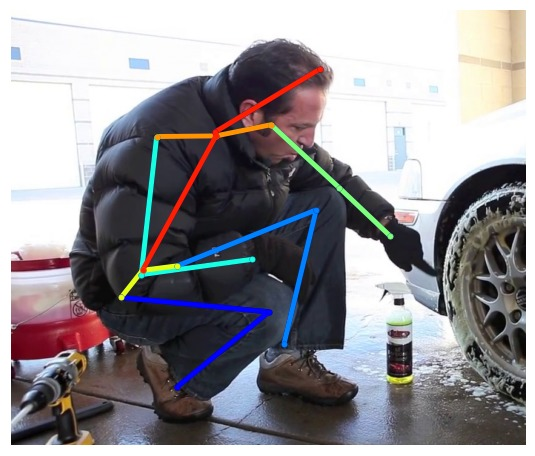
\includegraphics[height=\flowh]{Figures/pose/qualitative/pred-1}
    \hfill
    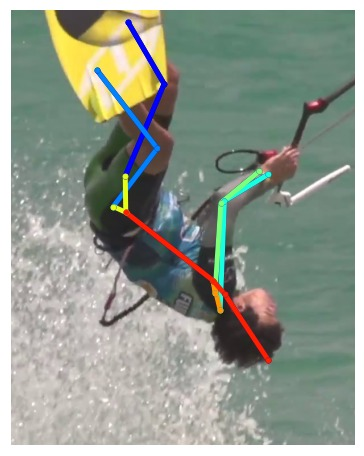
\includegraphics[height=\flowh]{Figures/pose/qualitative/pred-2}
    \hfill
    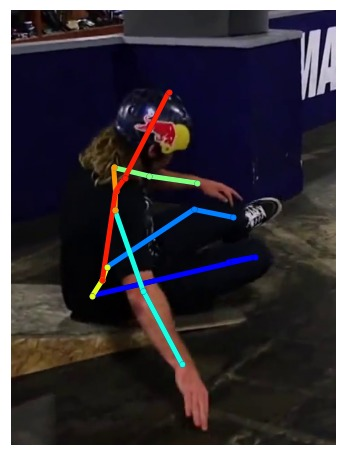
\includegraphics[height=\flowh]{Figures/pose/qualitative/pred-3}
    \hfill
    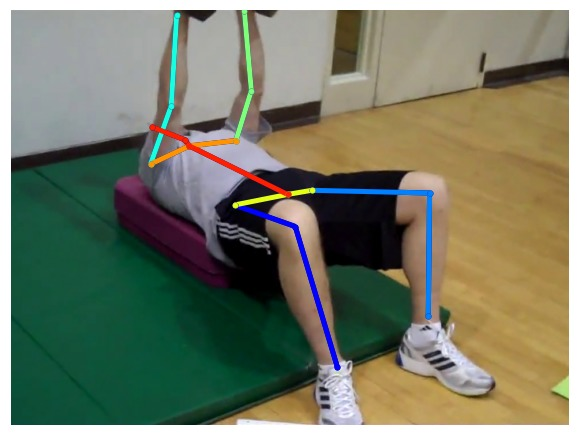
\includegraphics[height=\flowh]{Figures/pose/qualitative/pred-4}
    \hfill
    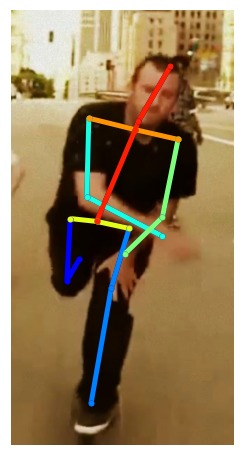
\includegraphics[height=\flowh]{Figures/pose/qualitative/pred-5}
    \hfill
    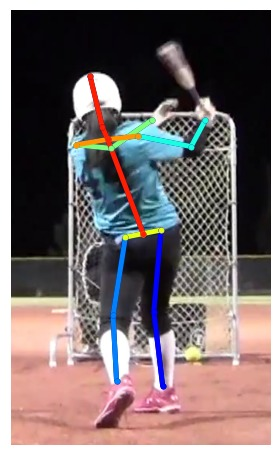
\includegraphics[height=\flowh]{Figures/pose/qualitative/pred-6}
    \hfill
    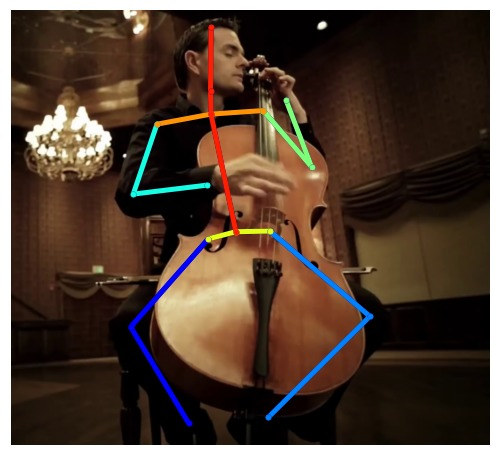
\includegraphics[height=\flowh]{Figures/pose/qualitative/pred-7}
    \\
    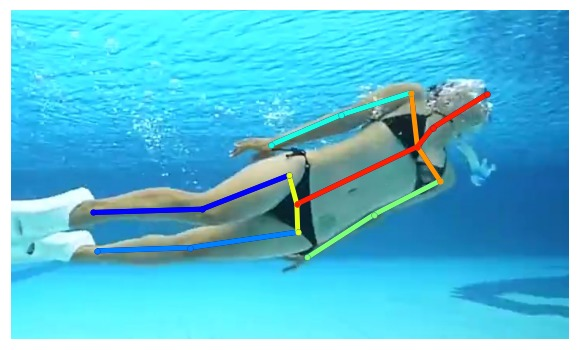
\includegraphics[height=\flowh]{Figures/pose/qualitative/pred-8}
    \hfill
    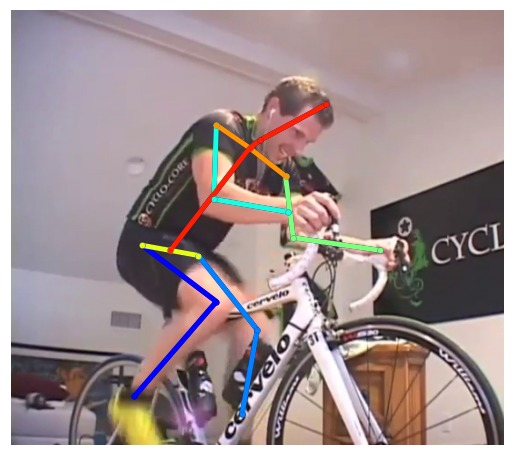
\includegraphics[height=\flowh]{Figures/pose/qualitative/pred-9}
    \hfill
    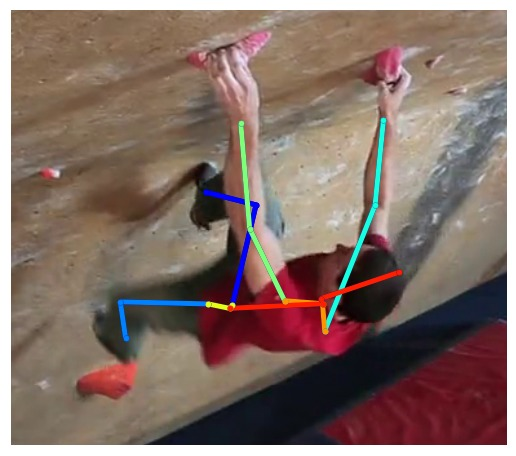
\includegraphics[height=\flowh]{Figures/pose/qualitative/pred-10}
    \hfill
    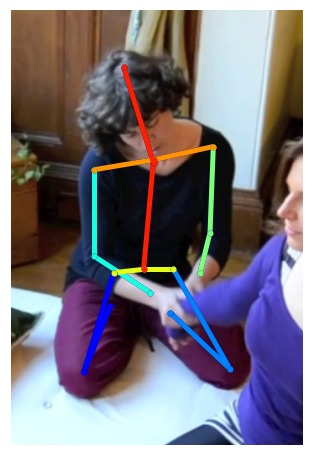
\includegraphics[height=\flowh]{Figures/pose/qualitative/pred-11}
    \hfill
    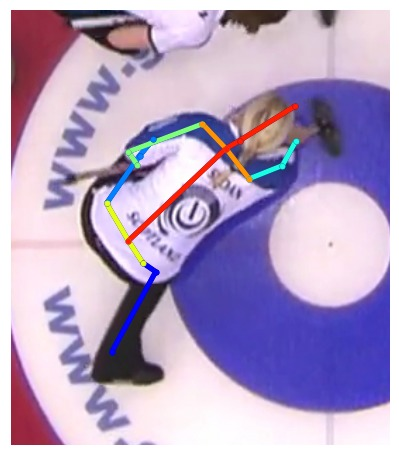
\includegraphics[height=\flowh]{Figures/pose/qualitative/pred-12}
    \hfill
    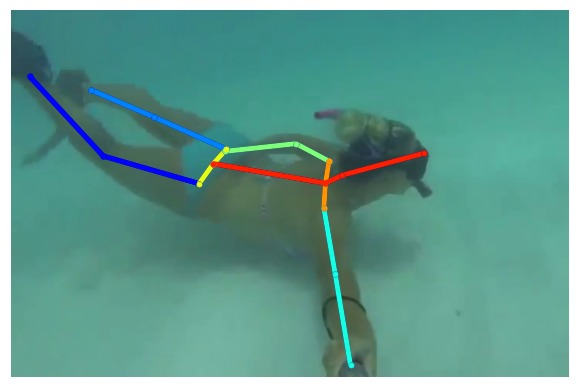
\includegraphics[height=\flowh]{Figures/pose/qualitative/pred-13}
    \\
    \newcommand{\flowhh}{0.27\columnwidth}
    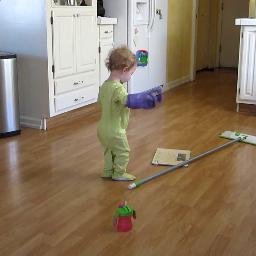
\includegraphics[height=\flowhh]{Figures/pose/qualitative/view/view_img_00}
    \hfill
    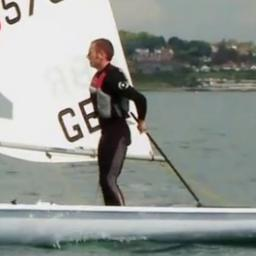
\includegraphics[height=\flowhh]{Figures/pose/qualitative/view/view_img_02}
    \hfill
    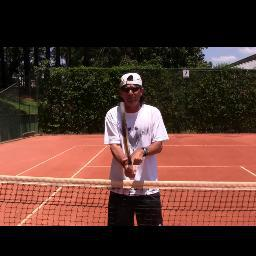
\includegraphics[height=\flowhh]{Figures/pose/qualitative/view/view_img_04}
    \hfill
    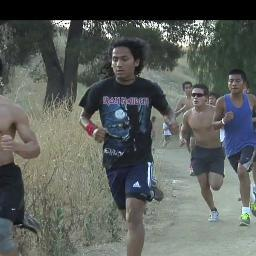
\includegraphics[height=\flowhh]{Figures/pose/qualitative/view/view_img_06}
    % \hfill
    % \includegraphics[height=\flowhh]{Figures/pose/qualitative/view/view_img_101}
    \hfill
    \includegraphics[height=\flowhh]{Figures/pose/qualitative/view/view_img_113}
    \hfill
    \includegraphics[height=\flowhh]{Figures/pose/qualitative/view/view_img_10}
    % \hfill
    % \includegraphics[height=\flowhh]{Figures/pose/qualitative/view/view_img_121}
    \hfill
    \includegraphics[height=\flowhh]{Figures/pose/qualitative/view/view_img_127}
    \\
    \includegraphics[height=\flowhh]{Figures/pose/qualitative/view/view_iuv_00}
    \hfill
    \includegraphics[height=\flowhh]{Figures/pose/qualitative/view/view_iuv_02}
    \hfill
    \includegraphics[height=\flowhh]{Figures/pose/qualitative/view/view_iuv_04}
    \hfill
    \includegraphics[height=\flowhh]{Figures/pose/qualitative/view/view_iuv_06}
    % \hfill
    % \includegraphics[height=\flowhh]{Figures/pose/qualitative/view/view_iuv_101}
    \hfill
    \includegraphics[height=\flowhh]{Figures/pose/qualitative/view/view_iuv_113}
    \hfill
    \includegraphics[height=\flowhh]{Figures/pose/qualitative/view/view_iuv_10}
    % \hfill
    % \includegraphics[height=\flowhh]{Figures/pose/qualitative/view/view_iuv_121}
    \hfill
    \includegraphics[height=\flowhh]{Figures/pose/qualitative/view/view_iuv_127}
    
    \caption{Examplar joints localisations on MPII and LSP test set. \textit{TOP 2 Rows}: Predictions of challenging poses in MPII and LSP test set. \textit{Bottom 3 row}: Examplar predictions of Landmarks, together with estimated dense correspondence IUV outputs are shown at each row correspondingly. Figure best viewed by zooming in.}
    \label{fig:qualitative_pose}
    \vspace{12pt}
\end{figure*}
\begin{table*}[t!]
\small
\begin{center}
\begin{tabular}{|l|r|r|r|r|r|r|r|r|r|}
\hline
\textbf{Methods} &\textbf{Head}   & \textbf{Shoulder} & \textbf{Elbow} & \textbf{Wrist} & \textbf{Hip}   & \textbf{Knee} & \textbf{Ankle} & \textbf{Total} & \textbf{AUC} \\
\hline
\hline
% Chu et al., CVPR'17           & 98.5  & 96.3  & 91.9  & 88.1  & 90.6  & 88.0 & 85.0 & 91.5 & 63.8 \\
\cite{newell2016stacked}       & 98.2  & 96.3  & 91.2  & 87.1  & \textbf{90.1}  & 87.4 & 83.6 & 90.9 & \textbf{62.9} \\
 \cite{bulat2016human} & 97.9  & 95.1  & 89.9  & 85.3  & 89.4  & 85.7 & 81.7 & 89.7 & 59.6 \\
 \cite{wei2016convolutional}          & 97.8  & 95.0  & 88.7  & 84.0  & 88.4  & 82.8 & 79.4 & 88.5 & 61.4 \\
 \cite{pishchulin16cvpr}   & 94.1  & 90.2  & 83.4  & 77.3  & 82.6  & 75.7 & 68.6 & 82.4 & 56.5 \\
\hline
DenseReg Cascade & \textbf{98.5}  & \textbf{96.4}  & \textbf{92.1}  & \textbf{88.2}  & 89.4  & \textbf{88.6} & \textbf{85.6} & \textbf{91.6} & 62.8 \\
\hline
\end{tabular}
\end{center}
\caption{Joints Localisation Accuracy on MPII dataset.}
\label{tab:mpii}
\vspace{12pt}
\end{table*}
\begin{table*}[t!]
\small
\begin{center}
\begin{tabular}{|l|r|r|r|r|r|r|r|r|r|}
\hline
\textbf{Methods} &\textbf{Head}   & \textbf{Shoulder} & \textbf{Elbow} & \textbf{Wrist} & \textbf{Hip}   & \textbf{Knee} & \textbf{Ankle} & \textbf{Total} & \textbf{AUC} \\
\hline\hline
 \cite{pishchulin2013poselet} & 87.2  & 56.7  & 46.7  & 38.0  & 61.0  & 57.5 & 52.7 & 57.1 & 35.8\\
 \cite{wei2016convolutional} & \textbf{97.8}  & 92.5  & 87.0  & 83.9  & 91.5  & 90.8 & 89.9 & 90.5 & 65.4\\
 \cite{bulat2016human}& 97.2  & 92.1  & 88.1  & 85.2  & \textbf{92.2}  & 91.4 & 88.7 & 90.7 & 63.4\\
 \cite{insafutdinov16ariv}& 97.4  & 92.7  & 87.5  & 84.4  & 91.5  & 89.9 & 87.2 & 90.1 & \textbf{66.1}\\
\hline
%HG+IUV &93.7  & 92.0  & 87.2  & 85.2  & 90.5  & 91.1 & 89.3 & 89.9 & 63.0\\
DenseReg Cascade& 94.7  & \textbf{93.4}  & \textbf{90.2}  & \textbf{88.2}  & 91.8  & \textbf{92.9} & \textbf{91.6} & \textbf{91.8} & 65.6\\
\hline
\end{tabular}
\end{center}
\caption{Joints Localisation Accuracy on LSP dataset.}
\label{tab:lsp}
\vspace{12pt}
\end{table*}

Since there are no dense correspondence results between a 3D human model and image pixels in literature, we demonstrate the performance of our system through visual results from our test-set partition of the UP dataset in Fig.\ref{fig:DenseReg_Human}. In order to provide quantitative experimental results in the following we evaluate DenseReg cascade architecture for the problem of articulated body pose estimation. 

\noindent\textbf{Evaluation Metrics} The accuracies reported follow the Percentage Correct Keypoints (PCK) measurement on LSP dataset. Normalised PCK measurement by the scale of head (PCKh) is used for MPII on both validation and test set. Note that the performance gap between validation and test set is due to the use of invisible parts in measuring the performance. That is, in the validation set we measured the performance making use of the invisible parts, while the test set protocol of MPII does not use the invisible parts when computing the evaluation metrics.

\noindent\textbf{Model Training} Our model is implemented using TensorFlow~\footnote{https://tensorflow.org}. 15k images from the training set mentioned above are used with augmentations. Each pose instance in the image was cropped to size $384 \times 384$. Cropped images are then randomly flipped, rotated by $\pm 30^{\degree} $ and rescaled by $0.75$ to $1.25$ before cropping to size $256 \times 256$. The model are trained with initial learning rate $1\times10^{-3}$ with exponential decay factor of $0.97$ at every $2$ epochs. The models were trained for 100 epochs before testing.

\begin{figure}[!h]
\centering
\includegraphics[width=0.89\linewidth]{Figures/DenseReg_Person-2}
\caption{Dense Correspondence for human body.}
\vspace{-0.25cm}
\label{fig:DenseReg_Human}
\end{figure}

\label{sec:pred_mpii_lsp}
\subsubsection{Joints Localisation on MPII \& LSP}

Results reported on MPII are obtained by using the proposed DenseReg cascade architecture. Table \ref{tab:mpii} provides a comparison of the proposed method with the state-of-the-art in MPII, while Table \ref{tab:lsp} provides a comparison with the state-of-the-art on LSP database.

Some qualitative results are collected in Fig~\ref{fig:qualitative} for the test sets of MPII and LSP. Top three rows show joint localization in challenging poses e.g. extreme viewing angles, challenging poses, occlusions, self occlusions and ambiguities. The bottom row demonstrates dense shape correspondence estimated on test images using the DenseReg cascade architecture.

 
%%%%%%%%%%%%%%%%%%%%%%%%%%%
%%%%%% EAR TRACKING %%%%%%%
%%%%%%%%%%%%%%%%%%%%%%%%%%%
\subsection{Ear Landmark Localization}
\label{sec:exp_ear}

We have also performed experiments on the human ear. We employ the $602$ images and sparse landmark annotations that were generated in a semi-supervised manner by Zhou et al.~\citep{Zhou_2016_CVPR}. Due to the lack of a 3D model of the human ear, we apply Thin Plate Splines to bring the images into dense correspondence and obtain the deformation-free space. We perform landmark localization following the same procedure as in Sec.~\ref{sec:exp_landmark_localization}.
%We split the images in $500$ for training and $102$ for testing.  
Quantitative results are detailed in the supplementary material, where we compare DenseReg, DenseReg + AAM and DenseReg + MDM with alternative DPM detector based initializations.  We observe that DenseReg results are highly accurate and clearly outperforms the DPM based alternative even without a deformable model. Examples for dense human ear correspondence estimated by our system  are presented in Fig.~\ref{fig:ears_examples}.


\begin{figure}[h]
\centering
\includegraphics[width=\linewidth]{Figures/ears3}
\caption{Exemplar pairs of deformation-free coordinates of dense landmarks on human ear.}
\label{fig:ears_examples}
\end{figure}

\subsubsection{Ear Shape Regression}

The deformation-free space for the ear shape template is visualized in Fig.~\ref{fig:earpoints}. The colouring of the qualitative results that are presented in the paper and this supplementary materials document are generated using these coordinates. On Table.\ref{tab:ears}, we provide failure rates and the Area Under Curve(AUC) measures based on the CED curve of the human ear landmark localization experiment, which were not provided in the paper due to space constraints. Further qualitative examples for regressed and ground-truth deformation-free ear coordinates are provided in Fig.~\ref{fig:ears_examples}.


\begin{figure}[h]
\centering
  \includegraphics[trim={3.1cm 8cm 0.35cm 7.3cm},width=0.7\linewidth]{Figures/EarPoints}
\caption{ Deformation-free space for the template ear shape. }
\label{fig:earpoints}
\end{figure}


%%%%%%%%%%%%%%%%%%%%%%%%%%%%%%%%%%%%%%%%
% \FloatBarrier
\begin{table}[h!]
\centering
\begin{tabular}{|l|c|c|}
\hline
\emph{Method} & \emph{AUC} & \emph{Failure Rate (\%)}\\
\hline\hline
\textbf{DenseReg + MDM} & \textbf{0.4842} & \textbf{0.98} \\
DenseReg       &  0.4150 &   1.96 \\
DenseReg + AAM &  0.4263 &  0.98 \\
DPM + MDM      &  0.4160 &  15.69 \\
DPM + AAM      &  0.3283 &  22.55 \\
\hline
\end{tabular}
\caption{Landmark localization results on human ear using 55 points. Accuracy is reported as the Area Under the Curve (AUC) and the Failure Rate of the Cumulative Error Distribution of the normalized RMS point-to-point error.}
\label{tab:ears}
\end{table}
